% \part{Java}

% ----------------------------------------------------------------------------
\section{Grundlagen}
\begin{frame}
\frametitle{Prozedurale Programmierung mit Java}
	\huge Grundlagen der Programmierung mit Java
\end{frame}

\begin{frame} 
	\frametitle{Java - Von der \"Ubersetzung zur Ausf\"uhrung}
	\center
	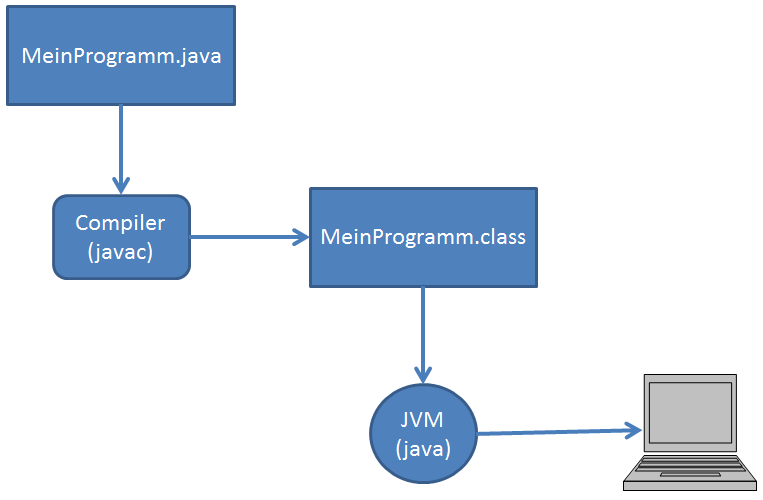
\includegraphics[width=0.8\textwidth,
	keepaspectratio=true]{bilder/java_process.png}
\end{frame}

\begin{frame}[fragile]
	\frametitle{Erste Schritte}
	\huge Erste Schritte
\end{frame}

\begin{frame}[fragile]
	\frametitle{Hello World!}
		\begin{columns}
		\begin{column}{0.5\textwidth}
			\small
			\begin{itemize}
			  \item Das Code-Listing zeigt unser erstes Java-Programm
			  \item Es wird mithilfe des Befehls ''javac HelloWorld.java'' 
			  übersetzt
			  \item Anschließend wird es mit ''java HelloWorld'' gestartet
			  \item mit ''javap -c HelloWorld'' lässt sich der Bytecode lesen
			\end{itemize}
			\normalsize
		\end{column}
		\begin{column}{0.5\textwidth}{\tiny \itshape Test.java}
			\begin{lstlisting}
						class HelloWorld {
							public static void main(String[] args){
								System.out.println("Hello World!");
							}
						}
			\end{lstlisting}
	\end{column}
	\end{columns}
\end{frame}

\begin{frame}[fragile]
	\frametitle{Aufbau von Java-Dateien}
	\begin{columns}
		\begin{column}{0.5\textwidth}
			\small
			\begin{itemize}
			  \item Jede .java Datei enth\"alt eine Klassendefinition
			  \item Wichtig: \\
			  		Dateiname = Klassenname
			  \item Klassen enthalten Methoden
			  \item Methoden enthalten Anweisungen
			\end{itemize}
			\normalsize
		\end{column}
		\begin{column}{0.5\textwidth}{\tiny \itshape Test.java}
			\begin{lstlisting}
				//Klassendefinition
				class Test {
					// Der Methodenkopf
					void test(){
						//Eine Anweisung
						System.out.println("Dies ist ein Test");
					}
				}
			\end{lstlisting}
		\end{column}
	\end{columns}
\end{frame}

\begin{frame}[fragile]
	\frametitle{Aufbau von Java-Dateien}
	\begin{columns}
		\begin{column}{0.5\textwidth}
			\small
			\begin{itemize}
			  \item Programm besteht (meistens) aus mehreren Klassen
			  \item Eine Klasse beeinhaltet eine Main-Methode
			  \item JVM startet Main-Methode
			  \item Programm endet nach Ablauf der Main-Methode
			\end{itemize}
			\normalsize
		\end{column}
		\begin{column}{0.5\textwidth}{\tiny \itshape TestMitMain.java}
			\begin{lstlisting}
				class TestMitMain {
					public static void main(String[] args){
						System.out.println("Dies ist ein Test");
					}
				}
			\end{lstlisting}
		\end{column}
	\end{columns}
\end{frame}

\subsection{Grundbegriffe}
\begin{frame}[fragile]
	\frametitle{Grundbegriffe}
	\huge Grundbegriffe
\end{frame}

\begin{frame}[fragile]
	\frametitle{Begrifflichkeiten}
	\begin{itemize}
	  \item Variablen und Konstanten
	  	\begin{itemize}
			\item Eine Variable ist ein mit Namen versehener Speicherplatz inklusive Inhalt
			\item Eine Konstante ist eine Variable, der nur genau einmal ein Wert
			zugewiesen werden darf
	    \end{itemize}
	  \item Datentypen
	 	\begin{itemize}
			\item Kombination aus Wertebereich und dazugehörigen Operationen
			\item Beispiel Ganzzahl: 	\\Wertebereich = $2^{32}$, 
										\\Operationen = Addition,Subtraktion\ldots
	    \end{itemize}
	  \item Operatoren
	  	\begin{itemize}
			\item Bestimmen wie mit Variablen, Konstanten und Literalen umgegangen wird
	    \end{itemize}
	 \end{itemize}
\end{frame}

\begin{frame}[fragile]
	\frametitle{Begrifflichkeiten}
	\begin{itemize}
	 \item Anweisungen
	  	\begin{itemize}
			\item Verarbeitungsvorschrift in imperativem Programm
			\item Durch Ausführung einer Anweisung werden Daten oder Adressen verarbeitet
			\item Verändert den Programmzustand
			\item Wichtige Anweisungstypen sind Variablendeklaration, Zuweisung,
			Auswahl, Schleife, Block\ldots
			\item Anweisungsfolge = Sequenz
			\item Einfachste Form besteht in Java lediglich aus ';'
	    \end{itemize}
	  \item Ausdrücke
	  	\begin{itemize}
			\item Verknüpfung von Variablen, Konstanten, Literalen oder anderen
			Ausdrücken durch Operatoren
			\item Werden in bestimmter Reihenfolge ausgewertet und haben Wert
			\item Einfachste Form besteht lediglich aus Konstante/Variable
			\item Wird in Java durch Abschluss mit Semikolon zu Anweisung 
	    \end{itemize}
	 \end{itemize}
\end{frame}

\subsection{Datentypen}
\begin{frame}[fragile]
	\frametitle{Datentypen}
	\huge Datentypen
\end{frame}

\begin{frame}[fragile]
	\frametitle{Datentypen}
	\small
	\begin{itemize}
	  \item Java enth\"alt 8 primitive Datentypen
	  \item Primitive Datentypen sind keine Objekte
	\end{itemize}
	\begin{table}
	\begin{tabular}{l|l|l}
			Name & Wertebereich & Standard\\ \hline
			char & Unicode-Zeichen & u0000 \\
			byte  & -128 bis 127 & 0 \\ 
			short & -32768 bis 32767 & 0 \\
			int & -2147483648 bis 2147483647 & 0 \\
			long & $-2^{63}$ bis $2^{63}-1$ & 0 \\
			float & +/-3.40282347*1038 & 0.0 \\
			double & +/-1.79769313486231570*10308 & 0.0 \\
			boolean& false, true & false \\
	\end{tabular}
	\end{table}
	\normalsize
\end{frame}

\begin{frame}[fragile]
	\frametitle{Zeichen}
	Der primitive Datentyp ''char''
	\begin{columns}
		\begin{column}{0.5\textwidth}
			\begin{itemize}
			  \item speichert Zeichen aus der Unicode-Zeichentabelle
			  \item 2 Byte (16 Bit) groß
			  \item jedes Zeichen besitzt einen code
			\end{itemize}
		\end{column}
		\begin{column}{0.5\textwidth}
		\begin{lstlisting}
				char zeichen;
				zeichen = 'a';
				zeichen = 97;
		\end{lstlisting}
		\end{column}
	\end{columns}
\end{frame}

\begin{frame}[fragile]
	\frametitle{Zeichen}
	\center
	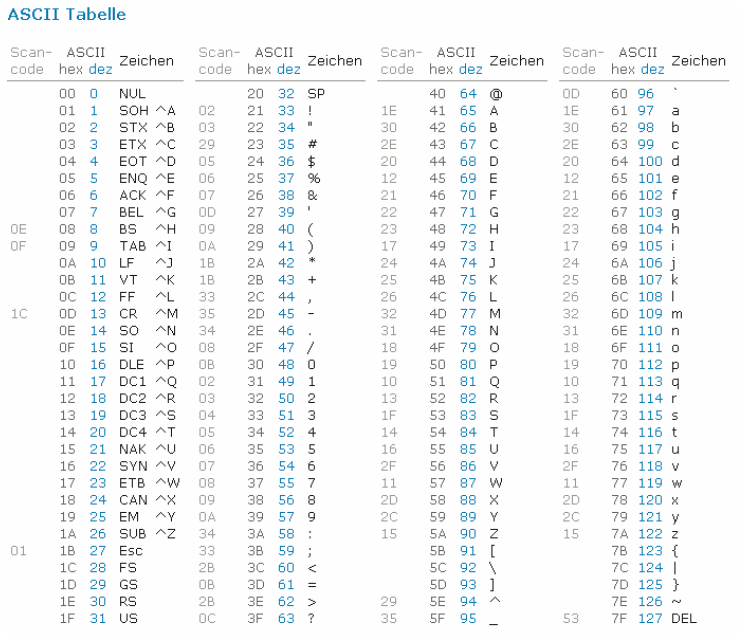
\includegraphics[width=0.95\textwidth,
	keepaspectratio=true]{bilder/ascii_table.png}
\end{frame}

\begin{frame}[fragile]
	\frametitle{Ganzzahlige Datenypen}
			\begin{itemize}
			  \item byte
			  \begin{itemize}
			    \item für sehr kleine Zahlen
			  	\item 1 Byte (8 Bit) groß
			  	\item Fängt bei Über- oder Unterschreitung des Wertebereichs wieder von
			  	vorn an
			  \end{itemize}
			  \item short
			  \begin{itemize}
			    \item für kleine Zahlen
			  	\item 2 Byte (16 Bit) groß
			  	\item Fängt bei Über- oder Unterschreitung des Wertebereichs wieder von
			  	vorn an
			  \end{itemize}
			\end{itemize}
\end{frame}

\begin{frame}[fragile]
	\frametitle{Ganzzahlige Datenypen}
			\begin{itemize}
			  \item int
			  \begin{itemize}
			    \item für gewöhnliche Zahlen
			  	\item 4 Byte (32 Bit) groß
			  	\item Fängt bei Über- oder Unterschreitung des Wertebereichs wieder von
			  	vorn an
			  \end{itemize}
			  \item long
			  \begin{itemize}
			    \item für sehr große Zahlen
			  	\item 8 Byte (64 Bit) groß
			  	\item Fängt bei Über- oder Unterschreitung des Wertebereichs wieder von
			  	vorn an
			  \end{itemize}
			\end{itemize}
\end{frame}

\begin{frame}[fragile]
	\frametitle{Fließkommazahlen}
			\begin{itemize}
			  \item float
			  \begin{itemize}
			    \item für gewöhnliche Fließkommazahlen
			  	\item 4 Byte (32 Bit) groß
			  	\item Fängt bei Über- oder Unterschreitung des Wertebereichs wieder von
			  	vorn an
			  	\item indikator: f (float x = 0.6f)
			  \end{itemize}
			  \item double
			  \begin{itemize}
			    \item für größere Fließkommazahlen
			  	\item 8 Byte (64 Bit) groß
			  	\item Fängt bei Über- oder Unterschreitung des Wertebereichs wieder von
			  	vorn an
			  	\item indikator: d (double x = 0.6d)
			  \end{itemize}
			\end{itemize}
\end{frame}

\begin{frame}[fragile]
	\frametitle{Boolesche Datentypen}
			\begin{itemize}
			  \item boolean
			  \begin{itemize}
			    \item für Wahrheitswerte
			    \item kann Wahr (true) oder Falsch (false) annehmen
			  	\item 1 Byte (8 Bit) groß
			  \end{itemize}
			\end{itemize}
\end{frame}

\subsection{Variablen}
\begin{frame}[fragile]
	\frametitle{Variablen}
	\huge Variablen
\end{frame}

\begin{frame}[fragile]
	\frametitle{Variablen}
	\begin{itemize}
	  \item Speichern Werte
	  \item Können gelesen und geschrieben werden
	  \item Namen bestehen aus
	  \begin{itemize}
	  	\item Buchstaben
	  	\item Ziffern  
	  	\item Unterstrich
	  \end{itemize}
	  \item Konstanten in Großbuchstaben
	  \item Variablen sollten mit Kleinbuchstaben beginnen (anschließend
	  Camel-Case)
	  \item Keine Schlüsselwörter als Namen
	\end{itemize}
\end{frame}

\begin{frame}[fragile]
	\frametitle{Java Schlüsselwörter}
	\center
	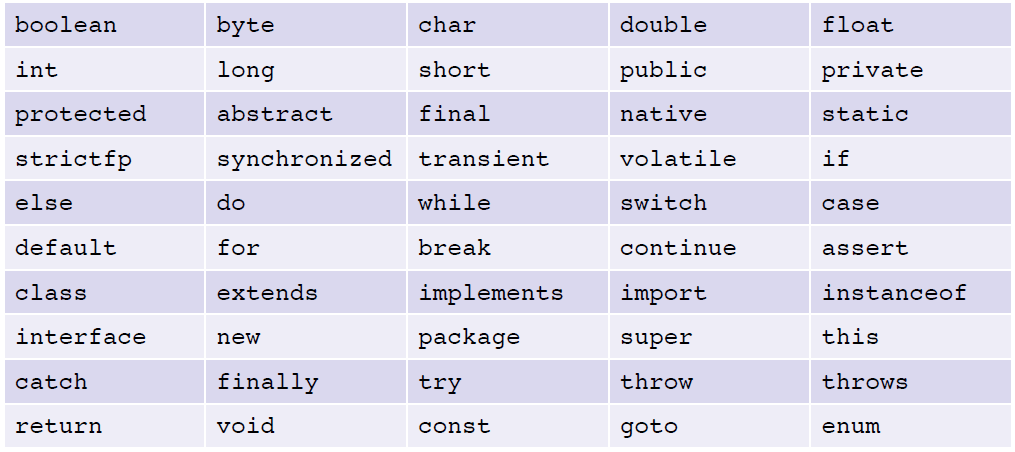
\includegraphics[width=0.99\textwidth,
	keepaspectratio=true]{bilder/keywords.png}\\
	\tiny (Übernommen von Herrn Prof. Dr. Dirk Wiesmann)
\end{frame}

\begin{frame}[fragile]
	\frametitle{Variablendeklaration}
	\begin{columns}
		\begin{column}{0.5\textwidth}
		\small
			Deklaration bedeutet\ldots
			\begin{itemize}
			  \item Variable benennen und dem Compiler bekanntmachen
			  \item Speicher für die Variable reservieren
			\end{itemize}
			Durch Initialisierung kann die Variable nun auf einen Anfangswert
			gesetzt werden.
		\end{column}
		\begin{column}{0.5\textwidth}
			\begin{lstlisting}
			// Syntax:
			// Datentyp VARNAME;
			
			// Variablen einzeln deklarieren
			int i;
			int x;
			int y;
			
			// Diese Schreibweise ist auch gueltig
			int i, x, y;
			\end{lstlisting}
		\end{column}
	\end{columns}
\end{frame}

\begin{frame}[fragile]
	\frametitle{Variableninitialisierung}
	\begin{columns}
		\begin{column}{0.5\textwidth}
			\small
			Initialisierung bedeutet\ldots
			\begin{itemize}
			  \item Variablendeklaration um eine Zuweisung ergänzen
			  \item die deklarierte Variable mit einem Wert zu befüllen
			\end{itemize}
			Der Wert einer Konstante darf nach der Initialisierung nicht mehr
			geändert werden
		\end{column}
		\begin{column}{0.5\textwidth}
			\begin{lstlisting}
			// Variablen einzeln deklarieren
			int i = 20;
			int x = 10;
			int y = i + x;
			
			// Diese Schreibweise ist auch gueltig
			int i = 20, x = 10, y = i+x;
			
			// Auch getrennt moeglich
			int a;
			a = 100;
			\end{lstlisting}
		\end{column}
	\end{columns}
\end{frame}

\begin{frame}[fragile]
	\frametitle{Typen von Variablen}
	\begin{columns}
		\begin{column}{0.5\textwidth}
			\small
				Es gibt in Java drei Arten von Variablen
					\begin{enumerate}
					  \item Klassenvariablen
					  \item Lokale Variablen
					  \item Instanzvariablen (OOP)
					\end{enumerate}
		\end{column}
		\begin{column}{0.5\textwidth}
			\begin{lstlisting}
				class Variablen {
					
					//Klassenvariable
					static boolean bool = true; 
					
					//Instanzvariable
					int i = 5; 
					
					public static void main(String[] args){ 
						
						//lokale Variable
						int i = 1;
						
					}
				}
			\end{lstlisting}
		\end{column}
	\end{columns}
\end{frame}
 
\begin{frame}
	\frametitle{Variablen}
	\begin{block}{Lebensdauer}
		\begin{itemize}
			 \item Klassenvariablen: Gesamte Programmlaufzeit
			 \item Lokale Variablen: Bis zum Ende des Methodenaufrufs
			 \item Instanzvariablen: Existenz des Objekts (OOP)
		\end{itemize}
	\end{block}
	\begin{exampleblock}{Sichtbarkeit}
		\begin{itemize}
			 \item Klassenvariablen: Innerhalb der Klasse
			 \item Lokale Variablen: Innerhalb eines Blocks
			 \item Instanzvariablen: Innerhalb des Objekts (OOP)
		\end{itemize}
	\end{exampleblock}
\end{frame} 

\begin{frame}[fragile]
	\frametitle{Casting}
	\begin{columns}
		\begin{column}{0.5\textwidth}
			\small
			\begin{itemize}
				\item Java kann Typen implizit casten
				\item Entwickler kann Typen explizit casten
				\item Casten in gr\"o"seren Datentyp geht implizit
				\item Casten in kleineren Datentyp explizit\\
						da Informationsverlust!
			\end{itemize}
		\end{column}
		\begin{column}{0.5\textwidth}
			\begin{lstlisting}
				int i = 10;
				
				// Cast in groesseren Typ 
				// kein Problem
				long l = i;
				
				// Cast in kleineren Typ explizit
				short s = (short) i;
			\end{lstlisting}
		\end{column}
	\end{columns}
\end{frame}

\begin{frame}
	\frametitle{Aufgaben}
	\begin{enumerate}
	  \item Weisen sie in der Main-Methode die Zahl 25 einer ganzzahligen Variable
	  zu, anschließend:
	  \begin{enumerate}
	    \item Geben Sie die Variable in der Form: ''Wert: 25'' aus
	    \item Geben Sie $25/5$, $25/3$, $25/3.0$ aus
	  \end{enumerate} 
	  \item Deklarieren sie die short-Variable ''einShort'' und initialisieren Sie
	  sie mit 4096, anschließend casten Sie die Variable in den Datentyp ''byte'' und
	  geben Sie die Zahl aus, was fällt auf?
	\end{enumerate}
\end{frame}

\subsection{Operatoren/Ausdrücke}
\begin{frame}[fragile]
	\frametitle{Operatoren und Ausdrücke}
	\huge Operatoren und Ausdrücke
\end{frame}

\begin{frame}[fragile]
	\frametitle{Arten von Operatoren}
	Die drei wichtigsten Operatorgruppen sind
	\begin{itemize}
	  \item Arithmetische Operatoren
	  \item Logische Operatoren
	  \item Zuweisungsoperatoren
	\end{itemize}
	Je nach Programmiersprache existieren weitere Operatoren
	(Inkrement-/Dekrement-/Bit-Operatoren).
\end{frame}

\begin{frame}[fragile]
	\frametitle{Unterteilung nach Anzahl der Operanden}
	Jeder Operator wird auf eine bestimmte Anzahl von Operanden angewendet. 
	Dadurch entsteht eine weitere Unterteilung:
	\begin{itemize}
	  \item Unäre Operatoren = 1 Operand, \\der hinter dem Operator folgt
	  \item Binäre Operatoren = 2 Operanden, \\Infix-Notation in Java
	  \item Tertiäre Operatoren = 3 Operanden
	\end{itemize}
\end{frame}

\begin{frame}[fragile]
	\frametitle{Auswertungsreihenfolge von Operatoren}
	Auswertungsreihenfolge ergibt sich aus 2 Faktoren:
	\begin{itemize}
	  \item Priorität des Operators\\
	  z.B. ''Punkt-vor-Strich''
	  \item Assoziativität des Operators = Bindung zwischen gleichwertigen
	  Operatoren\\
	  z.B: Ausdruck mit arithmetischen Operatoren der gleichen
	  Priorität wird von links nach rechts ausgewertet.
	\end{itemize}
	Durch Klammerung von Teilausdrücken kann die Auswertungsreihenfolge
	erzwungen werden.
\end{frame}

\begin{frame}[fragile]
	\frametitle{Operatoren und Ausdr\"ucke}
	Operatoren f\"ur numerische Datentypen:
	\begin{table}
	\begin{tabular}{l|l|l}
	Name & Erl\"auterung \\ \hline
			- & Subtraktion, neg. Vorzeichen \\
			* & Multiplikation \\
			/ & Division \\
			\% & Modulo \\
			++ & Pr\"a -/ Postinkrement \\
			-{}- & Pr\"a -/ Postdekrement \\
	\end{tabular}
	\end{table}
\end{frame}

\begin{frame}[fragile]
	\frametitle{Operatoren und Ausdr\"ucke}
	Vergleichsoperatoren
	\begin{table}
		\begin{tabular}{l|l}
			Name & Erl\"auterung  \\ \hline
			== & Gleich \\
			!= & Ungleich \\
			\textless & Kleiner \\
			\textgreater & Gr\"o"ser \\
			\textless= & Kleiner gleich \\
			\textgreater= & Gr\"o"ser gleich \\
		\end{tabular}
	\end{table}
\end{frame}

\begin{frame}[fragile]
	\frametitle{Operatoren und Ausdr\"ucke}
	Logische Operatoren
	\begin{table}
		\begin{tabular}{l|l}
			Name & Erl\"auterung  \\ \hline
			\&\&  & UND (Shortcircuit) \\
			$\mid\mid$ & ODER (Shortcircuit) \\
			! & NICHT \\
			\& & UND \\
			$\mid$ & ODER \\
			\textasciicircum & Exklusiv ODER \\
		\end{tabular}
	\end{table}
\end{frame}

\begin{frame}[fragile]
	\frametitle{Assoziativität}
	\center
	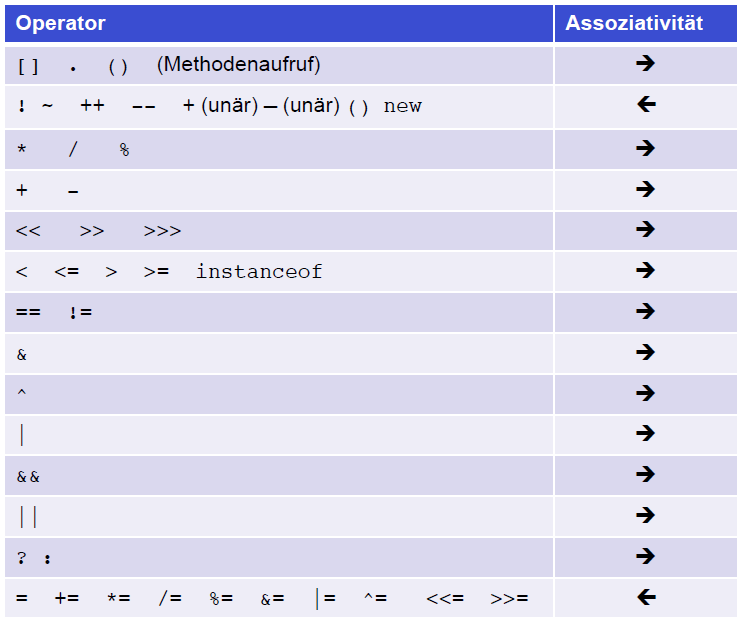
\includegraphics[width=0.9\textwidth,
	keepaspectratio=true]{bilder/assoz.png}\\
	\tiny (Übernommen von Herrn Prof. Dr. Dirk Wiesmann)
\end{frame}

\begin{frame}
	\frametitle{Aufgaben}
	\begin{enumerate}
	  \item Erstellen Sie ein Programm zur Multiplikation zweier Zahlen, die im
	  Programm einen festen Wert zugewiesen bekommen.
	  \item Verbessern Sie dieses Programm, indem mit Hilfe der Klasse ''Tastatur''
	  nun Zahlen über die Konsole eingegeben werden können.
	  \item Schreiben Sie ein Programm, dass den Benzinverbrauch eines Autos in
			Litern je 100 Kilometer errechnet. Als Eingabe benötigt das Programm den
			Benzinverbrauch in Litern und die gefahrenen Kilometer. Der Verbrauch pro 100
			Kilometer ergibt sich aus: $Liter * 100/km$.
	\end{enumerate} 
\end{frame}

\subsection{Kontrollstrukturen}
\begin{frame}[fragile]
	\frametitle{Kontrollstrukturen}
	\huge Kontrollstrukturen
\end{frame}

\begin{frame}[fragile]
	\frametitle{Kontrollstrukturen}
	  Kontrollstrukturen definieren die Reihenfolge in der Anweisungen ausgeführt
	  werden.
\end{frame}

\begin{frame}[fragile]
	\frametitle{Kontrollstrukturen - Block}
	\begin{columns}
		\begin{column}{0.5\textwidth}
			\small
			\begin{itemize}
			\item Fasst mehrere Anweisungen Zusammen
			\item Kann stehen wo auch einzelne Anweisungen stehen
			\item Kann geschachtelt werden
		\end{itemize}
		\end{column}
		\begin{column}{0.5\textwidth}
			\begin{lstlisting}
				{
					System.out.println("Ausgabe");
					System.out.println("Ausgabe");
				}
			\end{lstlisting}
		\end{column}
	\end{columns}
\end{frame}

\begin{frame}[fragile]
	\frametitle{Kontrollstrukturen - Fallunterscheidung}
	\begin{columns}
		\begin{column}{0.5\textwidth}
		\small
			\begin{itemize}
			  \item Bedingte Anweisung
			  \item Ausdruck ''Bedingung'' muss boolescher Ausdruck sein\\
			  d.h. \begin{itshape}true\end{itshape} oder
			  \begin{itshape}false\end{itshape}
			\end{itemize}
		\end{column}
		\begin{column}{0.5\textwidth}
			\begin{lstlisting}
				if(Bedingung){
					System.out.println("Die Bedingung ist True");
				}
			\end{lstlisting}
		\end{column}
	\end{columns}
\end{frame}

\begin{frame}[fragile]
	\frametitle{Kontrollstrukturen - Fallunterscheidung}
	\begin{columns}
		\begin{column}{0.5\textwidth}
			\small
			\begin{itemize}
			  \item Mehrfachauswahl
			  \item Auch hier: \\ 
			  Ausdr\"ucke ''Bedingung1'' \\
			  und ''Bedingung2'' m\"ussen boolesche Ausdr\"ucke sein\\
			  \item else-Zweig wird durchlaufen wenn kein Ausdruck wahr ist
			\end{itemize}
		\end{column}
		\begin{column}{0.5\textwidth}
			\begin{lstlisting}
				if(Bedingung1){
					System.out.println("Bedingung1 ist True");
				} else if(Bedingung2){
					System.out.println("Bedingung2 ist True");
				} else {
					System.out.println("Keine Bedingung ist True");
				}
				
				// If-Then-Else als 
				// ternaerer Operator
				Ausdruck = ( BedingungX ) ? Wahr : Falsch;
			\end{lstlisting}
		\end{column}
	\end{columns}
\end{frame}

\begin{frame}[fragile]
	\frametitle{Kontrollstrukturen - Fallunterscheidung}
	\begin{columns}
		\begin{column}{0.5\textwidth}
			\small
			\begin{itemize}
			  \item Mehrfachauswahl
			  \item Ausdruck vom Typ:\\
			  byte, short, char, int
			  \item Nach case darf genau 1 Konstante stehen
			  \item Wenn keine passende Konstante 
			  dann ''default'' Anweisung (wenn vorhanden)
			  \item Ohne break: \\
			  ausf\"uhren aller Anweisungen ab \"Ubereinstimmung
			  \item ''break'' ist syntaktisch nicht erforderlich
			\end{itemize}
		\end{column}
		\begin{column}{0.5\textwidth}
			\begin{lstlisting}
				switch(Ausdruck){
					
					case konst1:
						Anweisung1;
						break;
						
					case konst2:
						Anweisung2;
						break;
						
					default:
						Anweisung3;
						break;
						
				}
			\end{lstlisting}
		\end{column}
	\end{columns}
\end{frame}

\begin{frame}[fragile]
	\frametitle{Kontrollstrukturen - Schleifen}
	\begin{columns}
		\begin{column}{0.5\textwidth}
		\small
			\begin{itemize}
			  \item Kopfgesteuerte Schleife
			  \item Pr\"uft Ausdruck zu Beginn 
			\end{itemize}
		\end{column}
		\begin{column}{0.5\textwidth}
			\begin{lstlisting}
				while (Bedingung){
					Anweisung1;
					...
					Anweisungn;
				}
			\end{lstlisting}
		\end{column}
	\end{columns}
\end{frame}

\begin{frame}[fragile]
	\frametitle{Kontrollstrukturen - Schleifen}
	\begin{columns}
		\begin{column}{0.5\textwidth}
		\small
			\begin{itemize}
			  \item Fu"sgesteuerte Schleife
			  \item Pr\"uft Ausdruck am Ende der Schleife 
			\end{itemize}
		\end{column}
		\begin{column}{0.5\textwidth}
			\begin{lstlisting}
				do{
					Anweisung1;
					...
					Anweisungn;
				}while (Bedingung);
			\end{lstlisting}
		\end{column}
	\end{columns}
\end{frame}

\begin{frame}[fragile]
	\frametitle{Kontrollstrukturen - Schleifen}
	\begin{columns}
		\begin{column}{0.5\textwidth}
		\small
			\begin{itemize}
				  \item Z\"ahlschleife
				  \item Auch Kopfgesteuert
				  \item ''Initial'' wird vor 1. Durchlauf ausgewertet
				  \item ''Bedingung'' wird vor jedem Durchlauf ausgewertet
				  \item ''Inc/Dec'' wird nach jedem Durchlauf ausgewertet
				\end{itemize}
			\end{column}
		\begin{column}{0.5\textwidth}
			\begin{lstlisting}
				for(Initial; Bedingung; Inc/Dec)
				{
					Anweisung1;
					...
					AnweisungN;
				}
			\end{lstlisting}
		\end{column}
	\end{columns}
\end{frame}

\begin{frame}
	\frametitle{Aufgaben}
	\begin{enumerate}
	  \item Lassen Sie ein Rechteck von 10*10 Zeichen mit Sternchen ausfüllen
	  \item Erstellen Sie einen Taschenrechner, bei dem der Benutzer zwei
	  		Eingabewerte und die jeweilige Rechenoperation eingibt. Das Ergebnis der
	  		gewünschten Rechenoperation soll ermittelt und ausgegeben werden.
	  		Implementieren Sie dazu ein rudimentäres Menü, sodass der Nutzer den
	  		Taschenrechner solange nutzen kann, bis er das Programm beenden möchte.
	  		\\Nutzen Sie für die Eingabe die Klasse ''Tastatur''.
	  \item Erweitern Sie Ihr Programm um die Berechnung der Fakultät (n! = n * n-1
	  		* n-2 * 1; 0! = 1).
	  \item Berechnen Sie die Tabelle für das kleine Einmal-Eins für die Werte von
	  		1 bis 9 und geben das Ergebnis formatiert aus
	\end{enumerate}
\end{frame}

\begin{frame}
	\frametitle{Aufgaben}
	\begin{enumerate}
	  \item Geben Sie die Fibonacci-Zahlen von 1 bis n aus. Die Fibonacci-Folge ist
	 		eine Zahlenfolge, bei der sich die jeweils folgende Zahl durch Addition
	  		ihrer beiden vorherigen ergibt.\\
	  		Beispiele: $1+2=3$, $2+3=5$, $3+5=8$, $5+8=13$. 
	  		\\Die Formel lautet also: $F(n+2)=F(n+1) +F(n)$ mit $f(0) = 0$ und $f(1) =
	  		1$
	\end{enumerate}
\end{frame}

\begin{frame}
	\frametitle{Aufgaben}
	\begin{enumerate}
	  \item Erstellen Sie ein Programm zur Addition der ersten 15 ungeraden Zahlen
	 		(d. h. 1+3+5\ldots+15)
	  \item Verbessern Sie das Programm, indem die Endzahlen nun über die Konsole
	  		eingegeben werden können.
	  \item Erstellen Sie ein Programm zur Bestimmung der Primzahlen zwischen 1
	  		und 100.\\
	  		Die Idee: Jede Zahl n (1 $<$ n $<$ 100) wird durch alle Zahlen d (1 $<$ d
	  		$<$ n) dividiert. Das Ergebnis e wird mit d wieder multipliziert. Ist n =
	  		e*d, so ist n keine Primzahl.
	\end{enumerate}
\end{frame}

\subsection{Arrays}
\begin{frame}[fragile]
	\frametitle{Arrays}
	\huge Arrays
\end{frame}

\begin{frame}
	\frametitle{Arrays}
	\begin{itemize}
	  \item Array (Feld) fasst mehrere Variablen des gleichen Typs zusammen
	  \item Auf die einzelnen Elemente wird über einen Index zugegriffen
	  \item In Java ist ein Array ein Objekt (OOP)
	  		\begin{itemize}
	  		  \item Array-Variable ist Referenz (OOP)
	  		  \item Erzeugung zur Laufzeit (OOP)
	  		\end{itemize}
	  \item Größe des Feldes wird in ''length'' gespeichert
	\end{itemize}
\end{frame}

\begin{frame}[fragile]
	  \frametitle{Arrays}
	   \begin{columns}
		 \begin{column}{0.5\textwidth}
			  \small
			  \begin{itemize}
			    \item Der Index beginnt bei 0
			    \item Index muss vom Typ int sein
			    \item Die Feldgrenzen werden von Java überprüft
			    \item Bei Nicht-Einhaltung der Grenzen: Fehler!
			  \end{itemize}
	  	\end{column}
	  	\begin{column}{0.5\textwidth}
	  	 \small
			  Deklaration:\\
			  \begin{lstlisting}
			  // Reine Deklaration, Objekt existiert noch nicht
			  int[] intArray;
			  \end{lstlisting}
			  
			  Initialisierung:\\
			  \begin{lstlisting}
			  // Erzeugung des Array-Objekts auf dem Heap
			  intArray = new int[5];
			  
			  // Via Literale deklarieren und initialisieren:
			  int[] meinZweitesArray = {1,2,3,4,5};
			  \end{lstlisting}
			  
			  
			  Zuweisung von Werten:\\
			  \begin{lstlisting}
			  intArray[0] = 1;
			  intArray[1] = 2;
			  ...
			  \end{lstlisting}
	  	\end{column}
	  \end{columns}
\end{frame}

\begin{frame}[fragile]
	  \frametitle{Mehrdimensionale Arrays}
	   \begin{columns}
		 \begin{column}{0.5\textwidth}
			  \small
			  \begin{itemize}
			    \item Mehrdimensionales Array ist ein 
			    ''Array von Arrays''
			    \item Anzahl der Dimensionen ist unbegrenzt
			  \end{itemize}
	  	\end{column}
	  	\begin{column}{0.5\textwidth}
	  	 \small
			  Deklaration:\\
			  \begin{lstlisting}
			  int[][] multiDimIntArray;
			  \end{lstlisting}
			  
			  Initialisierung:\\
			  \begin{lstlisting}
			  multiDimIntArray = new int[2][3];
			  
			  // oder via literale
			  int[][] meinZweitesMultiDimArray = {{1,2,3},{4,5,6}};
			  \end{lstlisting}
			  
			  
			  Zuweisung von Werten:\\
			  \begin{lstlisting}
			  multiDimIntArray[0][0] = 1;
			  multiDimIntArray[0][1] = 2;
			  ...
			  \end{lstlisting}
	  	\end{column}
	  \end{columns}
\end{frame}

\begin{frame}
	\frametitle{Aufgaben}
	\begin{enumerate}
	  \item Entwerfen Sie ein Programm, das eine vorgegebene Anzahl Integer-Werte
	  		von der Tastatur einliest. Anschließend sollen zwei Funktionen den
	  		kleinsten und den größten eingegebenen Wert finden, die dann ausgegeben
	  		werden.
	  \item Schreiben Sie ein Programm, dass den Benutzer auffordert, zehn
	  		Schulnoten als Ganzzahlen einzugeben. Diese Zahlen sollen in einem Array
	  		gespeichert werden. Im Anschluss berechnen Sie die Summe
	  		sowie den Durchschnitt und geben diese aus.
	\end{enumerate}
\end{frame}

\begin{frame}
	\frametitle{Aufgaben}
	\begin{enumerate}
	  \item Schreiben Sie ein Java-Programm das Testet, ob eine Matrix ein
	 		magisches Quadrat ist. Dazu ist die Methode istMagisch(int[][] matrix) zu
	  		implementieren.\\(Ein magisches Quadrat ist eine n x n Matrix, in der die
	  		Summe aller Zeilen, Spalten sowie der beiden Diagonalen gleich ist.)
	  \item Entwickeln Sie eine kommandozeilenbasierte Version des Spiels
	  		''Tic-Tac-Toe''
	\end{enumerate}
\end{frame}

\subsection{Methoden}
\begin{frame}[fragile]
	\frametitle{Methoden}
	\huge Methoden
\end{frame}

\begin{frame}[fragile]
	  	\frametitle{Divide-and-Conquer (Teile und herrsche)}
		Divide-and-Conquer bedeutet große Probleme in kleinere Teilprobleme zu
		zerlegen.
		\begin{itemize}
		  \item Dieses Prinzip wird in Java durch Methoden ermöglicht.
		\end{itemize}
\end{frame}

\begin{frame}[fragile]
	  	\frametitle{Main-Methode und ausgelagerte Teilfunktionalität}
		\center
	    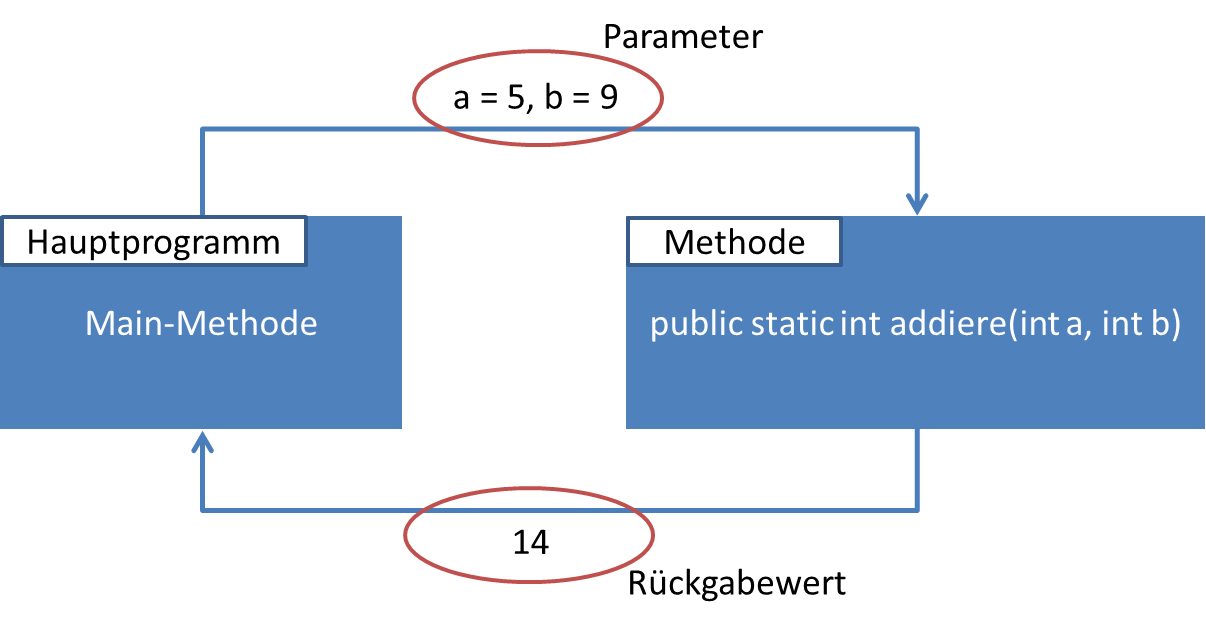
\includegraphics[width=1\textwidth,
	    keepaspectratio=true]{bilder/methode.png}
\end{frame}

\begin{frame}[fragile]
	  	\frametitle{Vorteile von Methoden}
		Vorteile:
		\begin{itemize}
		  \item Bessere Lesbarkeit des Programms
		  \item Wiederverwendung von Code
		  \item Fehler lassen sich schneller finden
		  \item Fehler müssen nur an einer Stelle behoben werden
		\end{itemize}
\end{frame}

\begin{frame}[fragile]
	  \frametitle{Methoden}
		 \begin{columns}
		 \begin{column}{0.5\textwidth}
			  \small
			  Methoden besitzen:
			  \begin{enumerate}
			  	\item Einen Methodennamen
			  	\item Anweisungsblock
			  	\item Lokale Variablen
			  	\item 0..* Parameter
			  	\item 0..1 R\"uckgabewerte (ohne R\"uckgabe: void)
			  	\item Wenn R\"uckgabewert dann ''return wert;''
			  	\item Zugriff auf Klassenattribute
			  	\item K\"onnen \"uberladen werden
			  \end{enumerate}
		 \end{column}
		 \begin{column}{0.5\textwidth}
		 	\begin{lstlisting}
		 		static Rueckgabetyp Methodenname (Typ Parameter, ...){
		 			Anweisung1;
		 			...
		 			AnweisungN;
		 			
		 			return wert;
		 		}
		 	\end{lstlisting}
		 \end{column}
		 \end{columns}
\end{frame}

\begin{frame}[fragile]
	  \frametitle{Beispielmethode: summieren}
			Beispiel einer Java-Methode
		 	\begin{lstlisting}
		 		static int summiere (int a, int b){
		 			int summe = a + b;
		 			return summe;
		 		}
		 	\end{lstlisting}
\end{frame}

\begin{frame}[fragile]
	\frametitle{Übergabe von Parametern}
			Parameter werden in Java nach dem Call-by-Value Prinzip übergeben.
			\\
			\begin{block}{Call-by-Value bedeutet\ldots}
				\begin{itemize}
				  \item das Kopieren der Übergabeparameter per Wert, 
				  \item ungeachtet ob es primitive Datentypen oder Objektreferenzen sind.
				\end{itemize}
			\end{block}
\end{frame}

\begin{frame}
	\frametitle{Aufgaben}
	\begin{enumerate}
	  \item Strukturieren Sie den implementierten Taschenrechner indem Sie
	  eigenständige Anweisungsblöcke in einzelne Methoden auslagern
	  \item Entwerfen Sie eine Funktion berechneUmfang(), die den
	  Umfang eines Kreises anhand des Radius berechnet.\\
	  pi = 3,141492 \\
	  Umfang = 2 * pi * Radius
	  \item Entwerfen Sie eine Funktion berechneFlaeche(), die die
	  Flaeche eines Kreises anhand des Radius berechnet.\\
	  pi = 3,141492 \\
	  Flaeche = $pi * Radius^2$
	\end{enumerate}
\end{frame}

\subsection{Rekursion}
\begin{frame}[fragile]
	\frametitle{Rekursion}
	\huge Rekursion
\end{frame}

\begin{frame}[fragile]
	  \frametitle{Rekursion}
	  \small
	  Eine Funktion ist rekursiv, wenn sie sich selbst aufruft.
	  \begin{itemize}
	    \item oftmals eine alternative zu Schleifen
	  \end{itemize}
	  \begin{center}
	  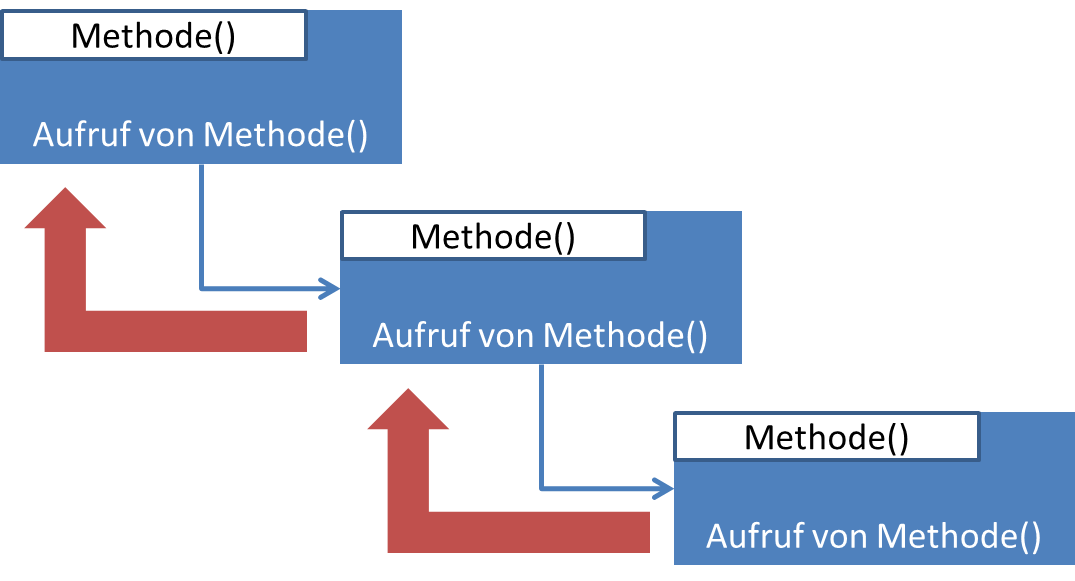
\includegraphics[width=0.75\textwidth,
	  keepaspectratio=true]{bilder/rekursion.png}
	  \end{center}
\end{frame}

\begin{frame}[fragile] 
	  \frametitle{Rekursive Berechnung der Fakultät}
		 \begin{columns}
		 \begin{column}{0.6\textwidth}
			  \small
			  Fakultät (!n) \\= Multiplikation der Zahlen von 1 bis n\\
			  Beispiel: 3! = 3 * 2 * 1
			  \begin{itemize}
			  	\item Die ersten (n-1) Faktoren des Produkts n! ergeben (n-1)!
			  	\begin{enumerate}
			  	  \item n! = (n-1)! $\cdot$ n falls n$\textgreater$1
			  	  \item n! = 1 falls n=1
			  	\end{enumerate}
			  	\item zu 1) \\n! zu berechnen wurde auf (n-1)! reduziert
			  	\item zu 2) \\Notwendig um Rekursion zu beenden
			  \end{itemize}
		 \end{column}
		 \begin{column}{0.4\textwidth}
		 	\begin{lstlisting}
		 		static int fakultaet (int n){
		 			int f;
		 			if(n > 1){
		 				f = fakultaet(n-1)*n;
		 			} else {
		 				f = 1;
		 			}
		 			return f;
		 		}
		 	\end{lstlisting}
		 \end{column}
		 \end{columns}
\end{frame}

\begin{frame}[fragile]
	  \frametitle{Analyse der Funktionsausführung}
	  \begin{center}
	  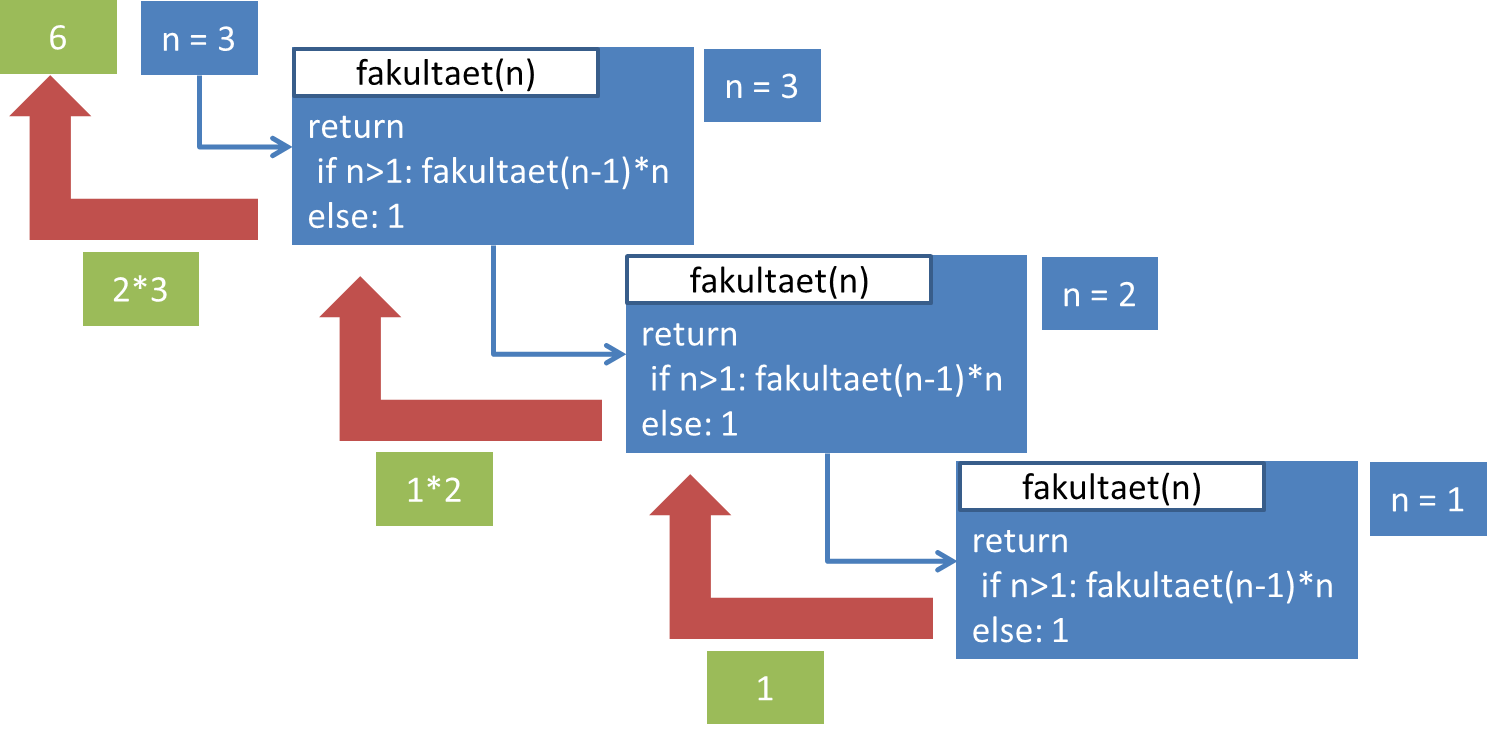
\includegraphics[width=1\textwidth,
	  keepaspectratio=true]{bilder/rekursion_konkret.png}
	  \end{center}
\end{frame}

\begin{frame}
	\frametitle{Aufgaben}
	\begin{enumerate}
	  \item Geben Sie die Fibonacci-Zahlen von 1 bis n rekursiv aus.
	  \item Schreiben Sie ein rekursives Programm, das den größten gemeinsamen
	  Teiler (GGT) zweier ganzer Zahlen berechnet.
	  \begin{enumerate}
	    \item ist Zahl1 == Zahl2 dann Ergebnis = Zahl1
		\item ist Zahl1  $>$ Zahl2 dann Ergebnis = ggT(Zahl1-Zahl2, Zahl2)
		\item ist Zahl1  $<$ Zahl2 dann Ergebnis = ggT(Zahl1, Zahl2-Zahl1)
	  \end{enumerate}
	  \item Der Springer darf beim Schach nur in L-Form bewegt werden. Ermitteln
	  		Sie rekursiv alle Züge, damit der Springer (von unten links angefangen)
	  		einmal alle Felder besucht ohne eines doppelt zu besuchen. Geben Sie
	  		anschließend das besuchte Schachfeld aus.
	\end{enumerate}
\end{frame}

\begin{frame}
	\frametitle{Aufgaben - Türme von Hanoi}
	  Lösen Sie das Problem der Türme von Hanoi rekursiv.
	  \begin{enumerate}
	  	\item n Scheiben unterschiedlichen Durchmessers, die der Größe nach
	  	sortiert übereinander liegen, bilden mit der größten Scheibe unten einen
	  	Turm. Der Turm soll von einem Platz 1 zu einem Platz 2 transportiert werden.
		\item Dabei steht ein Hilfsplatz 3 zur Verfügung.
 		\item Es darf jeweils nur die oberste Scheibe eines Turms bewegt werden.
 		\item Außerdem darf auf eine Scheibe nur eine kleinere Scheibe gelegt werden
	  \end{enumerate}
	  Implementieren Sie dazu die Funktion:\\
	  static void bewegeTurm(int n, int s, int z, int h)\\
	  Sie soll die notwendigen Scheibenbewegungen ausgeben, um einen Turm mit n
	  Scheiben vom Startplatz s zum Zielplatz z zu bewegen. Dazu existiert
	  ein zusätzlicher Hilfsplatz h.
\end{frame}

\begin{frame}
	\frametitle{Aufgaben - Türme von Hanoi}
	\center
	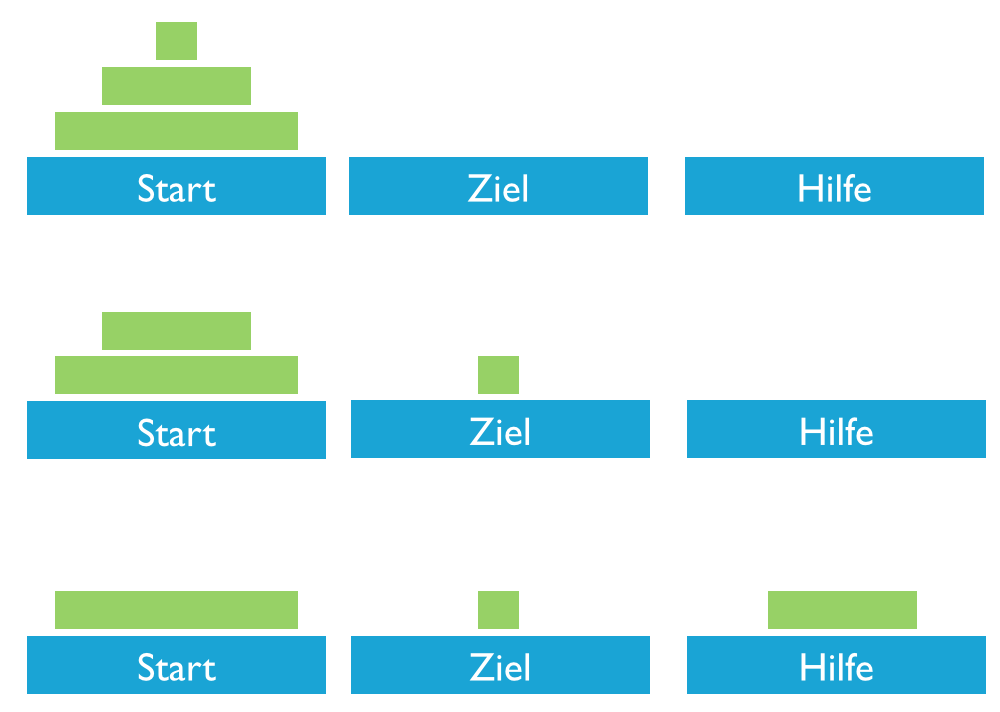
\includegraphics[width=1\textwidth, keepaspectratio=true]{bilder/hanoi1.png}
\end{frame}

\begin{frame}
	\frametitle{Aufgaben - Türme von Hanoi}
	\center
	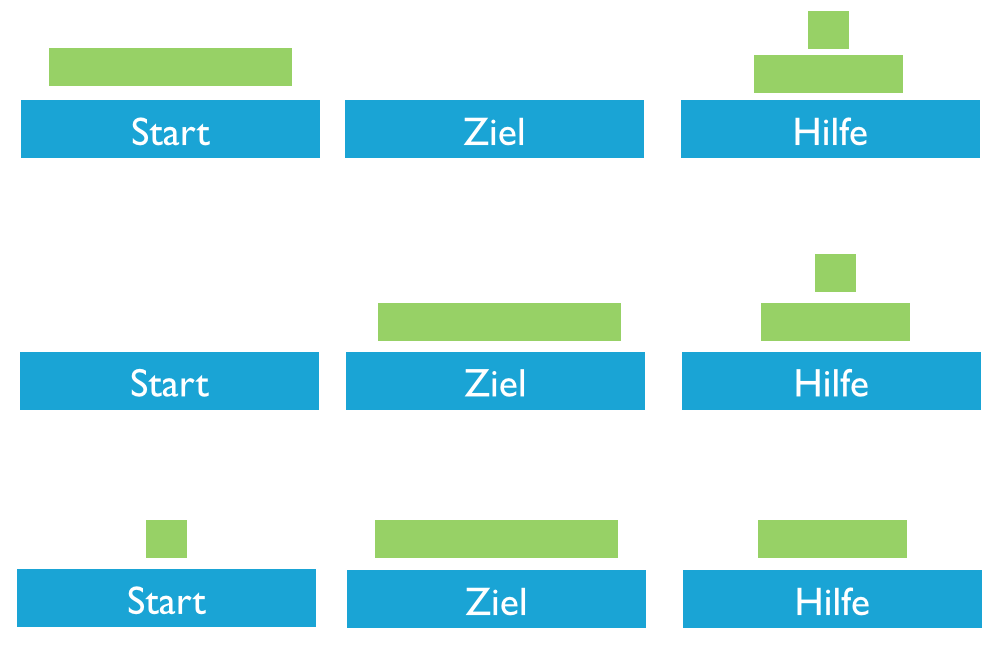
\includegraphics[width=1\textwidth, keepaspectratio=true]{bilder/hanoi2.png}
\end{frame}

\begin{frame}
	\frametitle{Aufgaben - Türme von Hanoi}
	\center
	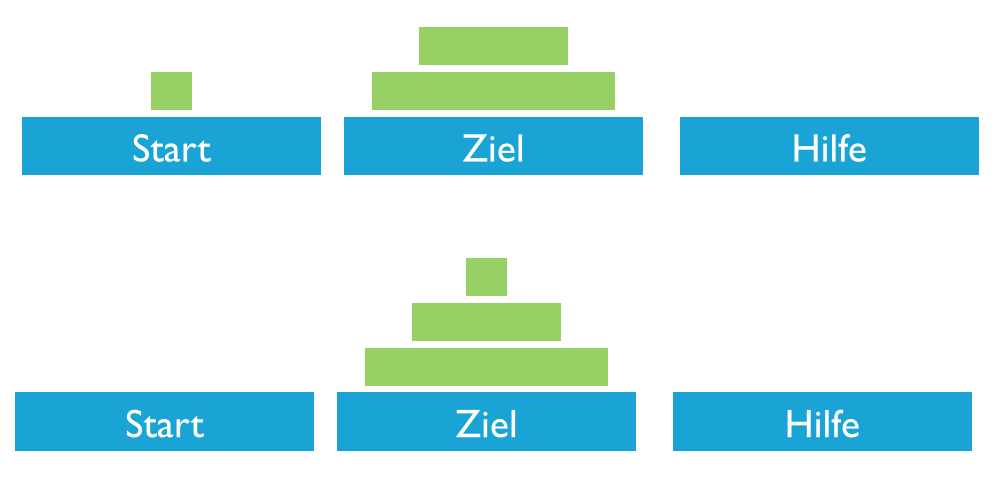
\includegraphics[width=1\textwidth, keepaspectratio=true]{bilder/hanoi3.png}
\end{frame}

\subsection{Strings}
\begin{frame}[fragile]
	\frametitle{Strings}
	\huge Strings
\end{frame}

\begin{frame}[fragile]
	  \frametitle{Strings}
		 \begin{columns}
		 \begin{column}{0.5\textwidth}
			  \small
			  \begin{itemize}
			    \item Strings sind Objekte (OOP)
			    \item Können ohne ''new'' angelegt werden
			    \item Konstruktoren existieren auch (OOP)
			    \item Strings sind immutable\\
			    (nicht veränderbar)
			    \item Ändern eines Zeichens erzeugt neuen
			    String
			    \item Vergleich mit equals-Methode
			  \end{itemize}
		 \end{column}
		 \begin{column}{0.5\textwidth}
		 	\begin{lstlisting}
		 		// Erstellen ohne ''new''
		 		String farbe = "rot";
		 		String farbe2 = "blau";
		 		
    			// Klasse hat viele Methoden
    			// Hier 3 Beispiele,
    			// mehr sind in der API-Doku

		 		// Gibt die Laenge zurueck
		 		int laenge = farbe.length();
		 		
		 		// Gibt das Zeichen 
		 		// an Position 2
		 		// zurueck
		 		// Wichtig: 1. Zeichen
		 		// steht an Position 0
		 		char c = farbe.charAt(2);
		 		
		 		// Ein Vergleich
		 		// Ergebnis: false
		 		farbe.equals(farbe2);
		 		
		 		// Noch ein Vergleich
		 		// Ergebnis: true
		 		"blau".equals(farbe2);
		 	\end{lstlisting}
		 \end{column}
		 \end{columns}
\end{frame}

\begin{frame}[fragile]
	  \frametitle{Strings}
		 \begin{columns}
		 \begin{column}{0.5\textwidth}
			  \small
			  \begin{itemize}
			    \item ''+''-Operator f\"ugt Strings zusammen
			    \item Andere Datentypen werden beim
			    Zusammenf\"ugen automatisch
			    in Strings umgewandelt
			  \end{itemize}
		 \end{column}
		 \begin{column}{0.5\textwidth}
		 	\begin{lstlisting}
		 		// String concat
		 		String a = "rot";
		 		String b = "blau";
		 		String c = "gruen";
		 		System.out.println(a+b+c);
		 		
		 		// Umwandlung in String
		 		int i = 10;
		 		String prefix = "Geld: ";
		 		String postfix = "Euro";
		 		String message = prefix + i + postfix;
		 		System.out.println(message);
		 	\end{lstlisting}
		 \end{column}
		 \end{columns}
\end{frame}

\begin{frame}
	\frametitle{Aufgaben}
	\begin{enumerate}
	  \item Wandeln Sie einen übergebenen String in Großbuchstaben um.
	  \\(Tipp: Schauen Sie in der Java-Doku)
	  \item Entwickeln Sie die Methode ''replace(String toReplace, String
	  replacement, String original)'' die die Zeichenkette ''toReplace'' in
	  ''original'' durch die Zeichenkette ''replacement'' ersetzt.
	  \item Sie bekommen eine aus Ganzzahlen bestehende Zeichenkette übergeben, die
	  durch Semikolon separiert sind. Berechnen Sie die Summe aus den Zahlen in der
	  Zeichenkette und geben Sie diese aus.
	\end{enumerate}
\end{frame}

\subsection{Enumerations}
\begin{frame}[fragile]
	\frametitle{Enumerations}
	\huge Enumerations
\end{frame}

\begin{frame}[fragile]
	\frametitle{Enumerations}
	\begin{columns}
		 \begin{column}{0.5\textwidth}
			  \small
				\begin{itemize}
				  \item Enumerations sind Aufzählungsobjekte (OOP).
				  \item Sie ermöglichen auf einfache und sichere Art und Weise
				 die Realisierung von Aufzählungen, als Alternative zu Konstanten.
				 \item Enums lassen sich erweitern, diese Funktionalität ist jedoch nicht
				 Teil der Veranstaltung.
				\end{itemize}
	 \end{column}
		 \begin{column}{0.5\textwidth}
		 	\begin{lstlisting}
		 		enum Wochentag {
		 			MONTAG, 
		 			DIENSTAG, 
		 			MITTWOCH, 
		 			DONNERSTAG, 
		 			FREITAG, 
		 			SAMSTAG,
		 			SONNTAG
		 		}
		 	\end{lstlisting}
		 \end{column}
	 \end{columns}
\end{frame}